
%LTeX: language=it
\subsection{UC 2 - Creazione e-mail} \label{sec:UC2}
    \begin{figure}[h]
        %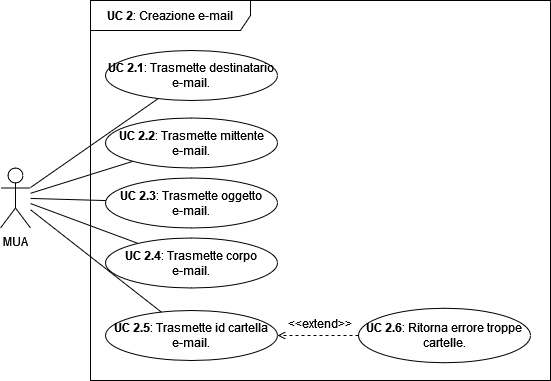
\includegraphics[width=0.85\textwidth]{sections/uc_imgs/UC02.png}
        \centering
        \caption{Diagramma UC 2}
    \end{figure}
    \begin{itemize}
        \item \textbf{Attore principale}: MUA;
        \item \textbf{Descrizione}: il MUA deve poter inviare una e-mail al destinatario indicato;
        \item \textbf{Precondizioni}: l’account che il MUA gestisce è registrato nel sistema, e ha un connessione aperta con il sistema ed è autenticato;
        \item \textbf{Postcondizioni}: l'e-mail è stata consegnata con successo al destinatario, ed è stata salvata nel sistema;
        \item \textbf{Scenario principale}:
            \begin{enumerate}
                \item il MUA trasmette il destinatario dell'e-mail (\hyperref[sec:UC2.1]{UC 2.1});
                \item il MUA trasmette il mittente dell'e-mail (\hyperref[sec:UC2.2]{UC 2.2});
                \item il MUA trasmette l'oggetto dell'e-mail (\hyperref[sec:UC2.3]{UC 2.3});
                \item il MUA trasmette il corpo dell'e-mail (\hyperref[sec:UC2.4]{UC 2.4});
                \item il MUA trasmette la cartella di appartenenza dell'email (\hyperref[sec:UC2.5]{UC 2.5});
                \item il sistema salva l'e-mail nel mailbox.
            \end{enumerate}
        \item \textbf{Inclusioni}: nessuna;
        \item \textbf{Generalizzazioni}: nessuna;
        \item \textbf{Estensioni}: 
            \begin{enumerate}[label=\alph*.]
                \item il sistema non riesce a creare l'e-mail perchè l'email ha troppe cartelle di destinazione:
                \begin{enumerate}[label=\arabic*.]
                    \item il sistema ritorna un errore al MUA di troppe cartelle (\hyperref[sec:UC2.6]{UC 2.6}).
                \end{enumerate}
            \end{enumerate}
    \end{itemize}

    \begin{figure}[h]
        %\includegraphics[width=0.75\textwidth]{sections/uc_imgs/UC02.X.png}
        \centering
        \caption{Diagramma sotto-casi UC 2.1}
    \end{figure}

    \subsubsection{UC 2.1 - Trasmette il destinatario dell'e-mail} \label{sec:UC2.1}
    \begin{itemize}
        \item \textbf{Attore}: MUA;
        \item \textbf{Descrizione}: il MUA invia al sistema il destinatario dell'e-mail;
        \item \textbf{Precondizioni}: il MUA sta usando la funzionalità di creazione di un'e-mail;
        \item \textbf{Postcondizioni}: il sistema conosce l'indirizzo di posta elettronica del destinatario dell'e-mail;
        \item \textbf{Scenario principale}:
            \begin{enumerate}
                \item il MUA trasmette il destinatario;
            \end{enumerate}
        \item \textbf{Inclusioni}: nessuna;
        \item \textbf{Generalizzazioni}: nessuna;
        \item \textbf{Estensioni}: nessuna;
    \end{itemize}

    \subsubsection{UC 2.2 - Trasmette il mittente dell'e-mail} \label{sec:UC2.2}
    \begin{itemize}
        \item \textbf{Attore}: MUA;
        \item \textbf{Descrizione}: il MUA invia al sistema il mittente dell'e-mail;
        \item \textbf{Precondizioni}: il MUA sta usando la funzionalità di creazione di un'e-mail;
        \item \textbf{Postcondizioni}: il sistema conosce l'indirizzo di posta elettronica del mittente dell'e-mail;
        \item \textbf{Scenario principale}:
            \begin{enumerate}
                \item il MUA trasmette il mittente;
            \end{enumerate}
        \item \textbf{Inclusioni}: nessuna;
        \item \textbf{Generalizzazioni}: nessuna;
        \item \textbf{Estensioni}: nessuna.
    \end{itemize}

    \subsubsection{UC 2.3 - Trasmette l'oggetto dell'e-mail} \label{sec:UC2.3}
    \begin{itemize}
        \item \textbf{Attore}: MUA;
        \item \textbf{Descrizione}: il MUA invia al sistema l'oggetto dell'e-mail;
        \item \textbf{Precondizioni}: il MUA sta usando la funzionalità di creazione di un'e-mail;
        \item \textbf{Postcondizioni}: il sistema conosce l'oggetto dell'e-mail;
        \item \textbf{Scenario principale}:
            \begin{enumerate}
                \item il MUA trasmette l'oggetto dell'e-mail;
            \end{enumerate}
        \item \textbf{Inclusioni}: nessuna;
        \item \textbf{Generalizzazioni}: nessuna;
        \item \textbf{Estensioni}: nessuna.
    \end{itemize}

    \subsubsection{UC 2.4 - Trasmette il corpo dell'e-mail} \label{sec:UC2.4}
    \begin{itemize}
        \item \textbf{Attore}: MUA;
        \item \textbf{Descrizione}: il MUA invia al sistema il corpo dell'e-mail;
        \item \textbf{Precondizioni}: il MUA sta usando la funzionalità di creazione di un'e-mail;
        \item \textbf{Postcondizioni}: il sistema conosce il corpo dell'e-mail;
        \item \textbf{Scenario principale}:
            \begin{enumerate}
                \item il MUA trasmette il corpo dell'e-mail;
            \end{enumerate}
        \item \textbf{Inclusioni}: nessuna;
        \item \textbf{Generalizzazioni}: nessuna;
        \item \textbf{Estensioni}: nessuna.
    \end{itemize}

    \subsubsection{UC 2.5 - Trasmette id cartella dell'e-mail} \label{sec:UC2.5}
    \begin{itemize}
        \item \textbf{Attore}: MUA;
        \item \textbf{Descrizione}: il MUA invia al sistema l'id della cartella di destinazione dell'e-mail;
        \item \textbf{Precondizioni}: il MUA sta usando la funzionalità di creazione di un'e-mail;
        \item \textbf{Postcondizioni}: il sistema conosce la cartella di destinazione dell'e-mail;
        \item \textbf{Scenario principale}:
            \begin{enumerate}
                \item il MUA trasmette l'id della cartella di destinazione dell'e-mail;
            \end{enumerate}
        \item \textbf{Inclusioni}: nessuna;
        \item \textbf{Generalizzazioni}: nessuna;
        \item \textbf{Estensioni}:             
        \begin{enumerate}[label=\alph*.]
            \item ci sono troppe cartelle di destinazione in cui salvare l'email:
            \begin{enumerate}[label=\arabic*.]
                \item il sistema ritorna un errore al MUA di troppe cartelle (\hyperref[sec:UC2.6]{UC 2.6}).
            \end{enumerate}
        \end{enumerate}
    \end{itemize}

    \subsubsection{UC 2.6 - Ritorna l'errore troppe cartelle} \label{sec:UC2.6}
    \begin{itemize}
        \item \textbf{Attore}: MUA;
        \item \textbf{Descrizione}: il MUA riceve l'errore che le cartelle di destinazione dell'email sono troppe;
        \item \textbf{Precondizioni}: il MUA ha trasmesso le cartelle di destinazione e-mail;
        \item \textbf{Postcondizioni}: il MUA viene notificato che le cartelle sono troppe;
        \item \textbf{Scenario principale}:
            \begin{enumerate}
                \item il sistema verifica il numero di cartelle;
                \item il sistema rileva che il numero di cartelle supera la soglia massima consentita;
                \item il sistema notifica il MUA dell'eccesso di cartelle nella e-mail;
            \end{enumerate}
        \item \textbf{Inclusioni}: nessuna;
        \item \textbf{Generalizzazioni}: nessuna;
        \item \textbf{Estensioni}: nessuna.
    \end{itemize}
